\section{Non-uniform costs, trees}
In this section we will be only concerned with the vertex-query variant of the problem. This is due to the fact that the edge variant is easily reducible to the vertex variant of the problem and this reduction preserves the approximation ratio (note that this reduces the problem to the version in which the last query may be omitted but all of the algorithms can be easily altered to consider this assumption). This is done by subdividing each edge $e$ with a new vertex $v_e$ of cost $c\br{v_e}=c\br{e}$. If we consider the average case criterion then we additionally set $w\br{v_e}=0$. It is immediate that the optimal decision tree for the this vertex query model instance can be used to obtain a decision tree for the original instance. To do so, simply replace each query to vertex $v_e$ with the query corresponding to $e$. 

\subsection{Worst case}

The problem for non-uniform is NP-hard even when restricted to spiders of diameter $6$ and binary trees.
A simple greedy heuristics which always queries the middle vertex of the graph achieves a $O\br{\log n}$-approximation \cite{Dereniowski2009ERankOfWTs}. However one can obtain better results. 
We begin with the following simple lemma which will become useful in few arguments:
\begin{lemma}\label{lemma:subtreeCost}
    Let $T'$ be a connected subtree of $T$. Then, $\OPT\br{T'}\leq\OPT\br{T}$.
\end{lemma}
The proof of this fact is trivial and will be left as an exercise for the reader.
\paragraph{A warm up: $O\br{\log n/\log\log n}$-approximation algorithm  for $T||V,c||C_{max}$}
This first algorithm is an adapted and simplified version of the algorithm due to \cite{Cicalese2016OnTSPwNonUniCost} for the edge query model.
\begin{theorem}
    There exists a polynomial time, $O\br{\log n/\log\log n}$-approximation algorithm for the $T||V,c||C_{max}$ problem .
    \begin{proof}
        
To construct a decision tree we will use the following exact procedure:
\begin{lemma}
    There exists a $O\br{2^nn}$ algorithm for $T||V,c||C_{max}$
    \begin{proof}
        The algorithm is a general version of the dynamic programming procedure for paths. We have that:
        $$
        \OPT_{max}\br{T} = \min_{v\in V\br{T}}\brc{c\br{v}+\max_{H\in T-v}\brc{\OPT_{max}\br{H}}}
        $$
        There are there are at most $O\br{2^n}$ different subtrees of $T$ to be checked. Additionally, and for each $v\in V\br{T}$ there are at most $\deg_T\br{v}$ possible responses to check in the inner $\max$ function. Therefore for each subproblem there are at most
        $
        \sum_{v\in V\br{T}}\deg_T\br{v} = 2m = 2n-2
        $
        comparison operations to be performed. As at each level of the recursion the algorithm considers all possible choices of the next queried vertex $v$ it returns the optimal decision tree for $T$ and the claim follows.
    \end{proof}
\end{lemma}
\begin{observation}\label{neighborsPathObservation}
    Let $D$ be a partial decision tree for tree $T$. Let $T'$ be a subtree of $T$. Let $Q$ be a set of all queries to vertices from $N_{T}\br{V\br{T'}}$ in $D$ such that every for every $q\in Q$: $q$ is queried before every vertex in $T'$. Then $D\angl{Q}$ is a path. 
    \begin{proof}
        Let $x\in N_{T}\br{V\br{T'}}$. In such case, for every vertex $v\in V\br{T-V\br{T'}-N_{T}\br{V\br{T'}}}$ the answer to a query to $v$ is always towards the same $u\in N_{T}\br{v}$, so until a vertex from $T'$ is queried, no query $q$ can partition vertices from $N_{T}\br{V\br{T'}}$ into disjoint subtrees of candidate vertices except when $q\in N_{T}\br{V\br{T'}}$. After a query to $q$, the only different response is when $x=q$, in which case no further queries are needed, so queries in $Q$ must belong to a path in $D$.
    \end{proof}
\end{observation}



Let $k=2^{\fl{\log\log n}+2}$.
The basic idea is as follows. The algorithm is recursive. Let $\mathcal{T}$ be the tree currently processed by the algorithm. If $n\br{T}\leq k$ then we use the exponential time algorithm to find the optimal solution in time $2^kk=\text{poly}\br{n}$.

If otherwise, to build a solution (see Algorithm \ref{cicaleseInspired}) we will firstly define a set $\mathcal{X}\subseteq V\br{\mathcal{T}}$ which will be of size at most $k$. We build $\mathcal{X}$ iteratively. Starting with an empty set we pick the centroid $x_1$ of $T$ which we add to $\mathcal{X}$. Then we take the forest $F=T-x$, find the largest $H\in F$, pick its centroid $x_2$ and append it to $\mathcal{X}$. We continue this in $F-H + \br{H-x_2}$ until $\spr{\mathcal{X}}=k$.
\begin{lemma}\label{lemma:componentSize}
    For every $H\in \mathcal{T}-\mathcal{X}$ we have that $n\br{H}\leq n\br{\mathcal{T}}/\log\br{n}$.
    \begin{proof}
        We prove by induction on $t$ that deleting first $2^t$ centroids from $T$ each connected components $H_t$ has size at most $n\br{H_t}\leq n\br{\mathcal{T}}/2^{t-1}$. For the case when $t=0$ we have that after 1 iteration every $H_1$ has size at most $n\br{T}/2\leq 2\br{n}$ so the base of induction is complete.

        Fix $t>0$ and by assume by the induction hypothesis that after $2^{t-1}$ iterations all
    \end{proof}
\end{lemma}

We also define set $\mathcal{Y}\subseteq V\br{\mathcal{T}}$ which consists of vertices in $\mathcal{X}$ and all vertices in $v\in \mathcal{T}\angl{X}$ such that $\deg_{T\angl{\mathcal{X}}}\br{v}\geq 3$.
Furthermore, we define set $\mathcal{Z}\subseteq V\br{\mathcal{T}}$ as a set consisting of vertices in $\mathcal{Y}$ and for every $u,v\in \mathcal{Y}$ such that $\mathcal{P}_{\mathcal{T}}\br{u, v}\neq\emptyset$ and $\mathcal{P}_{\mathcal{T}}\br{u, v}\cap \mathcal{Y}=\emptyset$ we add to $\mathcal{Z}$ the vertex $\argmin_{z\in \mathcal{P}_{\mathcal{T}}\br{u, v}}\brc{c\br{z}}$ (for example see Figure \ref{exampleTreeWithSetZ}). We then create an auxiliary tree $\mathcal{T}_{\mathcal{Z}}=\br{\mathcal{Z},\brc{uv|\mathcal{P}_{\mathcal{T}}\br{u, v}\cap \mathcal{Z}=\emptyset}}$ (for example see Figure \ref{exampleAuxTreeTZ}). The algorithm builds an optimal decision tree $D_{\mathcal{Z}}$ for $\mathcal{T}_{\mathcal{Z}}$ by applying the exponential time algorithm. Observe, that  $D_{\mathcal{Z}}$ is a  partial decision tree for $\mathcal{T}$, so we get that:
\begin{observation}\label{observation:CostDZinT}
    $\COST_{D_{\mathcal{Z}}}\br{\mathcal{T}_{\mathcal{Z}}}=\COST_{D_{\mathcal{Z}}}\br{\mathcal{T}}$.
\end{observation}
Then for each $H\in \mathcal{T}-\mathcal{Z}$ we recursively apply the same algorithm to obtain the decision tree $D_H$ and we hang it in $D_\mathcal{Z}$ below the unique last query to vertex in $N_{\mathcal{T}'}\br{H}$ (By Observation \ref{neighborsPathObservation}).

\begin{algorithm}
\caption{Main recursive procedure ($k$ is a global parameter)}\label{cicalese_inspired_pseudocode}
\SetKwFunction{FDecisionTree}{DecisionTree}
\SetKwProg{Fn}{Procedure}{:}{}
\Fn{\FDecisionTree{$\mathcal{T},c$}}{
    \If{$n\br{\mathcal{T}}\leq k$}{
    $D\gets$\FExact{$\mathcal{T},c$}.
    
    \Return $D$
    }
    $\mathcal{X}\gets\emptyset$.
    
    $\mathcal{F}\gets\brc{\mathcal{T}}$.
    
    \For{$1\leq i\leq k$ } 
        {
        \If{$\mathcal{F}=\emptyset$}{
            \textbf{break}
        }
        $H\gets\argmax_{H\in \mathcal{F}}\brc{n\br{H}}$.
        
        $x\gets$ the centroid of $H$.
        
        $\mathcal{X}\gets \mathcal{X}\cup\brc{x}$.
        
        $\mathcal{F}\gets \mathcal{F} \cup H-x$.
        }
    $\mathcal{Z}\gets\mathcal{Y}\gets\mathcal{X}\cup \brc{v\in \mathcal{T}\angl{\mathcal{X}}|\deg_{\mathcal{T}\angl{\mathcal{X}}}\br{v}\geq3}$.
    \tcp{Branching vertices in $\mathcal{T}\angl{X}$.}

    \ForEach{$u,v\in \mathcal{Y},\mathcal{P}_{\mathcal{T}}\br{u, v}\neq\emptyset,\mathcal{P}_{\mathcal{T}}\br{u, v}\cap \mathcal{Y}=\emptyset$}
    {
        $\mathcal{Z}\gets \mathcal{Z}\cup\brc{\argmin_{z\in \mathcal{P}_{\mathcal{T}}\br{u, v}}\brc{c\br{z}}}$. 
        \tcp{Lightest vertex on path $P_\mathcal{T}\br{u,v}$.}
    }
    
    $\mathcal{T}_{\mathcal{Z}}=\br{\mathcal{Z}, \brc{uv|\mathcal{P}_{\mathcal{T}}\br{u, v}\cap \mathcal{Z}=\emptyset}}$.
    
    $D\gets D_{\mathcal{Z}}\gets $\FExact{$\mathcal{T}_{\mathcal{Z}},c$}.

    \ForEach{$H\in \mathcal{T}-\mathcal{Z}$}
    {
        $D_H\gets$\FDecisionTree{$H,c$}.
        
        Hang $D_H$ in $D$ below the last query to a vertex $v \in N_{\mathcal{T}}\br{H}$.
    }
        
    \Return $D$
    
}
\end{algorithm}

\begin{lemma}\label{lemma:auxTreeSize}
    Let $\mathcal{T}_{\mathcal{Z}}$ be the auxiliary tree. Then, $\spr{V\br{\mathcal{T}_{\mathcal{Z}}}}\leq 4k-3$.
    \begin{proof}
        We firstly show that $\spr{\mathcal{Y}}\leq 2k-1$. We use induction of the centroids in $\mathcal{X}$. For $1\leq i\leq k$ let $x_i$ denote the $i$-th centroid added to $\mathcal{X}$. We will construct a family of sets $\mathcal{X}_1, \mathcal{X}_2,\dots, \mathcal{X}_{\spr{\mathcal{H}}}$ such that for any $1\leq t\leq \spr{\mathcal{X}}$: $\spr{\mathcal{X}_t}=t$ and $\mathcal{X}_{\spr{\mathcal{X}}}=\mathcal{X}$. For each $\mathcal{X}_t$ we will also construct a corresponding set $\mathcal{Y}_t$, ensuring $\mathcal{Y}_{\spr{\mathcal{X}}}=\mathcal{Y}$. We will build the sets $\mathcal{Y}_{t}$ to ensure that $\spr{\mathcal{Y}_t}\leq 2t-1$. 
        
        Let $\mathcal{X}_1=\brc{x_1}$, $\mathcal{Y}_1=\brc{x_1}$. This establishes the base case. Assume by induction on $t\geq1$ that $\spr{\mathcal{Y}_t}\leq 2t-1$ for some $t>1$. Let $\mathcal{X}_{t+1} =\mathcal{X}_{t}\cup \brc{x_{t+1}}$ and let $\mathcal{T}_t=\mathcal{T}\angl{\mathcal{X}_{t}}$ If $x_t\in V\br{\mathcal{T}_t}$ then $\mathcal{Y}_{t+1}=\mathcal{Y}_{t}\cup \brc{x_t}$. If otherwise let $y_t \in V\br{\mathcal{T}_t}$ be the unique vertex such that $P\br{x_t, y_t}\cap V\br{\mathcal{T}_t}=\emptyset$. Then $\mathcal{Y}_{t+1}=\mathcal{Y}_{t}\cup \brc{x_t, y_t}$. As by induction $\spr{\mathcal{Y}_{t}}\leq 2t-1$ and we add at most two vertices to it to obtain $\mathcal{Y}_{t+1}$ the induction step is complete.
        
        As paths between vertices in $\mathcal{Y}$ form a tree, at most $2k-2$ additional vertices are added to $\mathcal{Y}$ while constructing $\mathcal{Z}$ (at most one for each path) and the lemma follows.
    \end{proof}
\end{lemma}
\begin{lemma}\label{lemma:auxTreeCost}
    Let $\mathcal{T}_{\mathcal{Z}}$ be the auxiliary tree. Then, $\OPT\br{\mathcal{T}_{\mathcal{Z}}}\leq \OPT\br{\mathcal{T}}$.
    \begin{proof}
        Let $D^*$ be the optimal strategy for $\mathcal{T}\angl{\mathcal{Z}}$. We build a new decision tree $D_{\mathcal{Z}}'$ for $\mathcal{T}_{\mathcal{Z}}$ by transforming $D^*$: Let $u,v\in \mathcal{Y}$ such that $\mathcal{P}_{\mathcal{T}}\br{u, v}\neq\emptyset$ and $\mathcal{P}_{\mathcal{T}}\br{u, v}\cap \mathcal{Y}=\emptyset$. Let $q\in V\br{D^*}$ such that $q\in \mathcal{P}_{\mathcal{T}}\br{u, v}$ is the first query among vertices of $\mathcal{P}_{\mathcal{T}}\br{u, v}$. We replace $q$ in $D^*$ by the query to the distinct vertex $v_{u,v}\in \mathcal{P}_{\mathcal{T}}\br{u, v}\cap \mathcal{Z}$ and delete all queries to vertices $\mathcal{P}_{\mathcal{T}}\br{u, v}-v_{u,v}$ from $D^*$. By construction, $D_{\mathcal{Z}}'$ is a valid decision tree for $\mathcal{T}_{\mathcal{Z}}$ and as for every $z\in \mathcal{P}_{\mathcal{T}}\br{u, v}$: $c\br{v_{u,v}}\leq c\br{z}$ such strategy has cost at most $\COST_{D_{\mathcal{Z}}'}\br{\mathcal{T}_{\mathcal{Z}}}\leq \OPT\br{\mathcal{T}\angl{\mathcal{Z}}}$. We get:
        $$
        \OPT\br{\mathcal{T}_{\mathcal{Z}}}\leq \COST_{D_{\mathcal{Z}}'}\br{\mathcal{T}_{\mathcal{Z}}}\leq \OPT\br{\mathcal{T}\angl{\mathcal{Z}}}\leq \OPT\br{\mathcal{T}}
        $$

        where the first inequality is due to the optimality and the last inequality is due to the fact that $\mathcal{T}\angl{\mathcal{Z}}$ is a subtree of $\mathcal{T}$ (by Lemma \ref{lemma:subtreeCost}). The lemma follows.
    \end{proof}
\end{lemma}
\begin{lemma}
    Let $D_T$ be the solution returned by the algorithm. Then the approximation factor of such solution is bounded by 
    $
    \APP_T\br{D_T}\leq \log n/\log\log n
    $.
    \begin{proof}
        Let $\mathcal{T}$ be the tree processed at some level of the recursion and let $D_{\mathcal{T}}$ be the decision tree returned by the algorithm. The proof is by induction on the size of $\mathcal{T}$.  We claim that $\APP_{\mathcal{T}}\br{D_{\mathcal{T}}}\leq \max\brc{1, \log n\br{\mathcal{T}}/\log\log n}$. If $n\br{\mathcal{T}}\leq k$ then $D_{\mathcal{T}}$ is the optimal decision tree for $\mathcal{T}$ which establishes the base case. Let $n\br{\mathcal{T}} > k$ and assume that claim holds for every $t< n\br{\mathcal{T}}$. 
        By construction, we have that:
        \begin{align*}
        \APP_{D_{\mathcal{T}}}\br{\mathcal{T}}&=\frac{\COST_{D_{\mathcal{T}}}\br{\mathcal{T}}}{\OPT\br{\mathcal{T}}}\\
        &\leq \frac{\COST_{D_{\mathcal{Z}}}\br{\mathcal{T}}+\max_{H\in \mathcal{T}-\mathcal{Z}}\brc{C_{D_H}\br{H}}}{\OPT\br{\mathcal{T}}}\\
        &\leq 
        \frac{\COST_{D_{\mathcal{Z}}}\br{\mathcal{T}_{\mathcal{Z}}}}{\OPT\br{\mathcal{T}_{\mathcal{Z}}}}+\max_{H\in \mathcal{T}-\mathcal{Z}}\brc{\frac{C_{D_H}\br{H}}{\OPT\br{H}}}\\
        &\leq 1+\frac{\log\frac{n\br{\mathcal{T}}}{\log n\br{\mathcal{T}}}}{\log\log n}= \frac{\log n\br{\mathcal{T}}}{\log\log n}
        \end{align*}
        where the first inequality is by construction, the second is by usage of Observation \ref{observation:CostDZinT}, Lemma \ref{lemma:auxTreeCost} and Lemma \ref{lemma:subtreeCost} and the last inequality is due to the Lemma \ref{lemma:componentSize} and the induction hypothesis.
    \end{proof}
\end{lemma}
    Using the fact that the call to the exponential time procedure requires $O\br{2^{4k-3}\br{4k-3}}=\text{poly}\br{n}$ time (Due to Lemma \ref{lemma:auxTreeSize}), all other computations require polynomial time, and each $v\in V\br{T}$ belongs to $\mathcal{Z}$ at most once during the execution we get that the overall running time is polynomial in $n$.
    \end{proof}
\end{theorem}
In the above analysis we lose one factor of $\OPT$ per each level of recursion of which there are at most $O\br{\log n/\log\log n}$. Notice however, that we can allow some more loss (i. e. $c\cdot\OPT$) without affecting the asymptotical approximation factor. As it turns out it is possible to obtain a constant factor approximation for this problem in quasipolynomial time. This is the main idea behind the improvement of the approximation factor for this problem as in such case the size of the set $\mathcal{Z}$ may be greater and less recursion levels are needed which directly improves the approximation.
\paragraph{An $O\br{\sqrt{\log n}}$-approximation algorithm for $T||V,c||C_{max}$}
We begin with the following proposition \cite{dereniowski2017ApproxSsForGeneralBSinWTs} about the existence of QPTAS for $T||V,c||C_{max}$:
\begin{proposition}\label{QPTAS}
     For any $0 < \epsilon \leq 1$ there exists a $(1+\epsilon)$-approximation algorithm for the Tree Search Problem running in $2^{O\br{\frac{\log^2n}{\epsilon^2}}}$ time.
\end{proposition}
The algorithm and the proof of its correctness are very intricate and requires usage of an alternative notion of strategy. However, we rewrite it to use the language of the decision trees. Since the proof is involved for now we will use it as a black-box. The proof will be differed to a separate paragraph after the analysis below.

\begin{theorem}
    There exists a polynomial time, $O\br{\log n/\log\log n}$-approximation algorithm for the $T||V,c||C_{max}$ problem .
    \begin{proof}
    We use the same procedure as in the $O\br{\log n/\log\log n}$-approximation algorithm, however we set $k=2^{\fl{\sqrt{\log n}}+2}$ and we swap the exact procedure to the QPTAS with $\epsilon=1$. The analysis of the algorithm is largely the same except the evaluation of the cost of this solution.
    \begin{lemma}
        Let $D_T$ be the solution returned by the algorithm. Then the approximation factor of such solution is bounded by 
    $
    \APP_T\br{D_T}\leq 2\sqrt{\log n}
    $.
    \begin{proof}
        Let $\mathcal{T}$ be the tree processed at some level of the recursion and let $D_{\mathcal{T}}$ be the decision tree returned by the algorithm. The proof is by induction on the size of $\mathcal{T}$.  We claim that $\APP_{\mathcal{T}}\br{D_{\mathcal{T}}}\leq \max\brc{1, 2\log n\br{\mathcal{T}}/\sqrt{\log n}}$. If $n\br{\mathcal{T}}\leq k$ then $D_{\mathcal{T}}$ is the optimal decision tree for $\mathcal{T}$ which establishes the base case. Let $n\br{\mathcal{T}} > k$ and assume that claim holds for every $t< n\br{\mathcal{T}}$. 
        By construction, we have that:
        \begin{align*}
        \APP_{D_{\mathcal{T}}}\br{\mathcal{T}}&=\frac{\COST_{D_{\mathcal{T}}}\br{\mathcal{T}}}{\OPT\br{\mathcal{T}}}\\
        &\leq \frac{\COST_{D_{\mathcal{Z}}}\br{\mathcal{T}}+\max_{H\in \mathcal{T}-\mathcal{Z}}\brc{C_{D_H}\br{H}}}{\OPT\br{\mathcal{T}}}\\
        &\leq \frac{\COST_{D_{\mathcal{Z}}}\br{\mathcal{T}_{\mathcal{Z}}}}{\OPT\br{\mathcal{T}_{\mathcal{Z}}}}+\max_{H\in \mathcal{T}-\mathcal{Z}}\brc{\frac{C_{D_H}\br{H}}{\OPT\br{H}}}\\
        &\leq 2+\frac{2\log\frac{n\br{\mathcal{T}}}{\sqrt{\log n}}}{\sqrt{\log n}}= \frac{2\log n\br{\mathcal{T}}}{\sqrt{\log n}}
        \end{align*}
        where the first inequality is by construction, the second is by usage of Observation \ref{observation:CostDZinT}, Lemma \ref{lemma:auxTreeCost} and Lemma \ref{lemma:subtreeCost} and the last inequality is due to the Lemma \ref{lemma:componentSize} and the induction hypothesis.
    \end{proof}
\end{lemma}
    \end{proof}
\end{theorem}
\paragraph{QPTAS for the $T||V,c||C_{max}$ problem}
\begin{observation}\label{basicBoundsOnCost}
    Let $T$ be a tree such that $\spr{V\br{T}}> 1$ and $c:V\to \mathbb{R}^+$ be a normalized weight function. Then, $1\leq \OPT(T) \leq \fl{\log n}+1$.
\end{observation}

\paragraph{Constant factor approximation for monotonic query costs}

\paragraph{$O\br{\log\log n}$-approximation algorithm parametrized by the $k$-up-modularity of the cost function}

Let $s\in\mathbb{R}^+$. We define a \textit{heavy module} with respect to $s$ as $H\subseteq V\br{T}$ such that: $T[H]$ is connected, for every $v \in H$: $c\br{v}\geq s$ and $H$ is maximal - no vertex can be added to it without violating one of its properties. We then define the \textit{heavy module set} of $c$ in $T$ as: $HM_{T,c}\br{s}=\brc{H\subseteq V\br{T}|H \text{ is a heavy module w.r.t. } s}$ (abbreviated to $HM\br{s}$). Let $k\br{T,c}= \max_{s\in\mathbb{R}^+}\brc{\spr{HM_{T,c}\br{s}}}$. We say that a function $c$ is $k$\textit{-up-modular} in $T$, when $k\geq k\br{T,c}$. Whenever clear from the context we will use $k\br{T,c}$, $k\br{T}$, or $k$ to denote the lowest value such that $c$ is $k$-up modular in $T$. 

The notion of $k$-up-modularity is a direct generalization of the concept of up-monotonicity of the cost function. It is easy to see that in fact 1-up-modularity is equivalent to up-monotonicity. Observe that if $c$ is up-monotonic in $T$ then for every $s\in\mathbb{R}^+$: $T[V\br{T}-\brc{v\in V\br{T}: c\br{v}<s}]$ is connected and forms a single heavy module. Conversely, let $r=\argmax_{v\in V\br{T}}\brc{c\br{v}}$ and $u$ be any other vertex. If $c$ is 1-up-modular in $T$ then there is no vertex $v$ on path between $r$ and $u$ such that $c\br{v}<c\br{u}$. If otherwise then for any $s\in \br{v,u}$: $v$ does not belong to any heavy module but $u$ and $r$ do. As $v$ lays between them $\spr{HM\br{s}}>1$, a contradiction.

From now on we will again assume that all weights are normalized, so that the weight of the heaviest vertex is exactly 1. If not, the weights are scaled by dividing them by $\max_{v\in V\br{T}}\brc{w(v)}$.

The main idea of the algorithm is to divide vertices into \textit{cost levels} and process them in a recursive manner. At each level of the recursion the algorithm broadens the subset of vertices of $T$ having queries assigned to them. This continues until every $v\in T$ has a query to it scheduled. We consider the following intervals which we call \textit{cost levels}:
\begin{enumerate}
    \item Firstly, an interval $\left( 0,\frac{1}{\log n}\right]$.
    \item Then, each next interval $\mathcal{I}'=\left(a',b'\right]$ starts at the left endpoint of the previous interval $\mathcal{I}=\left(a,b\right]$, that is, $a'=b$ and ends with $b'=\min\brc{2b, 1}$. This results in the following sequence of intervals:
    $$\left(\frac{1}{\log n},\frac{2}{\log n}\right], \left(\frac{2}{\log n},\frac{4}{\log n}\right],\dots, \left(\frac{2^{\cl{\log\log n}-1}}{\log n},1\right]$$
\end{enumerate} 
After obtaining a solution for previous interval recursively, the next consecutive weight level $\mathcal{I}$ is processed by extending the strategy to contain all queries to vertices $v$ such that $c\br{v}\in \mathcal{I}$.
Once the last interval $\left(\frac{2^{\cl{\log\log n}-1}}{\log n},1\right]$ is processed the algorithm returns a valid decision tree for $T$. 

We are now ready to introduce the notions of heavy and light vertices (and queries to them). We say that a vertex $v$ (or the query to it) is \textit{heavy} with respect to the interval $\mathcal{I}=\left(a,b\right]$, when $c\br{v}>a$. If otherwise, i.e. $c\br{v}\leq a$ then, the vertex (and the query to it) is \textit{light} with respect to $\mathcal{I}$. Whenever clear from the context, we will omit the term "with respect to" and just call the vertices and queries heavy and light.


\begin{figure}[htbp]
    \begin{minipage}[t]{0.5\textwidth}
    \centering
    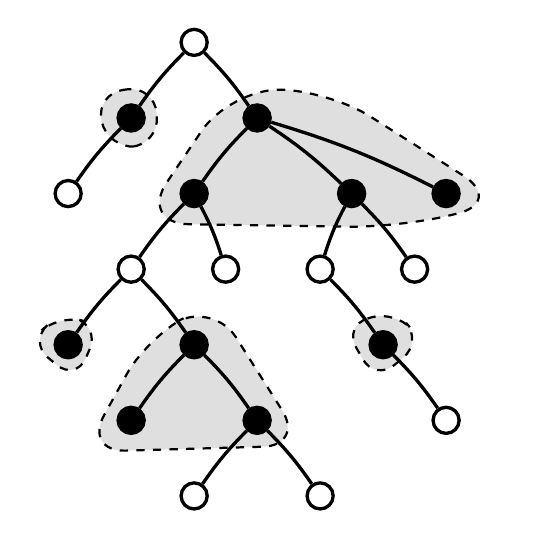
\begin{tikzpicture}[every node/.style={draw, very thick}, every path/.style={very thick}]
    
    \draw[dashed, thick, rounded corners = 10pt, fill= gray!25]
         (-1.25,5.75)  -- (-0.5,5.85)--  (-0.45,5.1) -- (-1.1,5.05) -- cycle;

    \draw[dashed, thick, rounded corners = 18pt, fill= gray!25]
        (0.45,5.8)  -- (1.7,5.8)-- (3.95,4.37) -- (2.6,4.05) -- (-0.7,4.1) -- cycle;
    \draw[dashed, thick, rounded corners = 9pt, fill= gray!25]
        (-2.1,2.6) -- (-1.7,2.95) -- (-1.2,2.8)  -- (-1.5,2.1) -- cycle;
        
    \draw[dashed, thick, rounded corners = 15pt, fill= gray!25]
         (-0.6,2.65) -- (0.25,3.1) -- (1.4,1.28) -- (-1.4,1.2) -- cycle;

    \draw[dashed, thick, rounded corners = 9pt, fill= gray!25]
        (1.9,2.8)  -- (2.55,3)  -- (2.9,2.6) -- (2.3,2.1) -- cycle;
    
    \node[circle, draw, fill=white] (1) at (0,6.4) {};
    
    \node[circle, draw, fill=black] (2) at (-0.8,5.44) {};
    \node[circle, draw, fill=black] (3) at (0.8,5.44) {};

    \node[circle, draw, fill=white] (4) at (-1.6,4.48) {};
    \node[circle, draw, fill=black] (5) at (0,4.48) {};
    \node[circle, draw, fill=black] (6) at (2.0,4.48) {};
    \node[circle, draw, fill=black] (7) at (3.2,4.48) {};
    
    \node[circle, draw, fill=white] (8) at (-0.8,3.52) {};
    \node[circle, draw, fill=white] (9) at (0.4,3.52) {};
    \node[circle, draw, fill=white] (10) at (1.6,3.52) {};
    \node[circle, draw, fill=white] (11) at (2.8,3.52) {};
    
    \node[circle, draw, fill=black] (12) at (-1.6,2.56) {};
    \node[circle, draw, fill=black] (13) at (0,2.56) {};
    \node[circle, draw, fill=black] (14) at (2.4,2.56) {};
    
    \node[circle, draw, fill=black] (15) at (-0.8,1.6) {};
    \node[circle, draw, fill=black] (16) at (0.8,1.6) {};
    \node[circle, draw, fill=white] (17) at (3.2,1.6) {};
    
    \node[circle, draw, fill=white] (18) at (0,0.64) {};
    \node[circle, draw, fill=white] (19) at (1.6,0.64) {};
    
    \draw[bend right=5] (1) to (2);
    \draw[bend left=5] (1) to (3);
    
    \draw[bend right=5] (2) to (4);
    \draw[bend right=5] (3) to (5);
    \draw[bend left=5] (3) to (6);
    \draw[bend left=5] (3) to (7);
    
    \draw[bend right=5] (5) to (8);
    \draw[bend left=5] (5) to (9);
    \draw[bend right=5] (6) to (10);
    \draw[bend left=5] (6) to (11);
    
    \draw[bend right=5] (8) to (12);
    \draw[bend left=5] (8) to (13);
    \draw[bend left=5] (10) to (14);
    
    \draw[bend right=5] (13) to (15);
    \draw[bend left=5] (13) to (16);
    \draw[bend left=5] (14) to (17);
    
    \draw[bend right=5] (16) to (18);
    \draw[bend left=5] (16) to (19);

    \end{tikzpicture}
\end{minipage}
    \begin{minipage}[t]{0.5\textwidth}
    \centering
    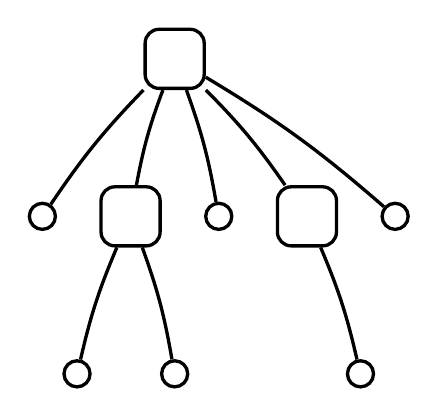
\begin{tikzpicture}[every node/.style={draw,rounded corners=5pt, very thick}, every path/.style={very thick}]
    
    \node[rectangle, minimum size=0.75cm, draw] (1) at (-0.56,10) {};
    
    \node[circle, draw] (2) at (-2.24,8) {};
    \node[rectangle, minimum size=0.75cm, draw] (3) at (-1.12,8) {};
    \node[circle, draw] (4) at (0,8) {};
    \node[rectangle, minimum size=0.75cm, draw] (5) at (1.12,8) {};
    \node[circle, draw] (6) at (2.24,8) {};
    
    \node[circle, draw] (7) at (-1.8,6) {};
    \node[circle, draw] (8) at (-0.56,6) {};
    \node[circle, draw] (9) at (1.8,6) {};
    
    \draw[bend right=5] (1) to (2);
    \draw[bend right=5] (1) to (3);
    \draw[bend left=5] (1) to (4);
    \draw[bend left=5] (1) to (5);
    \draw[bend left=5] (1) to (6);
    
    \draw[bend right=5] (3) to (7);
    \draw[bend left=5] (3) to (8);
    \draw[bend left=5] (5) to (9);

    \end{tikzpicture}
\end{minipage}
    \caption[Heavy module contraction]{Example of contracting 5 heavy modules. Black vertices represent heavy vertices, white vertices represent light vertices and square vertices represent vertices which were a parent of at least one heavy module before contraction.}\label{exampleHeavymoduleContraction}
\end{figure}
At last, we introduce the contraction operation.
Let $s>c\br{r\br{T}}$ and let $H$ be a heavy module with respect to $s$. Let $v$ be a parent of $r\br{T[H]}$ (observe that such a parent always exists as the tree is rooted at the lightest vertex and $s>c\br{r\br{T}}$).
A \textit{contraction} of a heavy module $H$ is an operation which consists of deleting all of the vertices in $H$ from $T$ and connecting every vertex $u$ which was a child of some vertex in $H$ to $v$ (note, that this definition slightly differs from the standard contraction, for example see Figure \ref{exampleHeavymoduleContraction}). This leads to the following simple observations:

\begin{observation}
\label{monotonicityOfOptContraction}
    Let $T'$ be a tree created by contraction of a heavy module $H$ in $T$. Then, $\OPT\br{T'}\leq \OPT\br{T}$.
\end{observation}
\begin{observation}\label{monotonicityOfKContracion}
    Let $T'$ be a tree created by contraction of a heavy module $H$ in $T$. Then, $k\br{T'}\leq k\br{T}$.
\end{observation}


We are ready to present the main recursive procedure. To avoid ambiguity, let $\mathcal{T}$ be the tree processed at some level of the recursion. Alongside $\mathcal{T}$, the algorithm takes as an input the interval $\left(a,b\right]$ such that for every $v\in \mathcal{T}$: $c\br{v}\leq b$. 
% For simplicity, we will say that vertices or modules are heavy when they are heavy with respect to $\left(a,b\right]$. 
The algorithm (see Algorithm \ref{createDecisionTree}) works in the following manner: 

\begin{algorithm}[H]
\caption{Main recursive procedure ($n$ is a global parameter)}
\label{createDecisionTree}
\SetKwFunction{FCreateDecisionTree}{CreateDecisionTree}
\SetKwFunction{FExtendDecTree}{ExtendDecTree}
\SetKwProg{Fn}{Procedure}{:}{}
\Fn{\FCreateDecisionTree{$\mathcal{T}$, $\left(a,b\right]$}}{
    \If{$b \leq \frac{1}{\log n}$ \textbf{or} for every $v \in \mathcal{T}$: $c\br{v} > a$}{
        \tcp{Every vertex in $\mathcal{T}$ is heavy}
        \Return a decision tree $D$ built by using the vertex ranking of $\mathcal{T}$\;
    }
    \Else{
        \tcp{There are light vertices in $\mathcal{T}$}
        Create $\mathcal{T}_C$ by contracting all heavy modules in $\mathcal{T}$\;
        
        $D_C \gets$\FCreateDecisionTree{$\mathcal{T}_C$, $\left(\frac{a}{2},a\right]$}\;
        
        $D \gets$\FExtendDecTree{$\mathcal{T}$, $D_C$, $\left(a,b\right]$}\tcp{Apply Proposition \ref{existanceOfExtensionAlgorithm}}
        \Return $D$\;
    }
}
\end{algorithm}


\begin{itemize}
    \item The base case happens whenever for every $v\in\mathcal{T}$: $c\br{v}\leq\frac{1}{\log n}$ or for every $v\in\mathcal{T}$: $c\br{v}>a$, i.e. every vertex is heavy. In such situation a solution is build by disregarding the costs of vertices and building a decision tree by using the vertex ranking of $\mathcal{T}$. 
    \item If otherwise, all heavy modules in $\mathcal{T}$ are contracted, forming a new tree $\mathcal{T}_C$ and a decision tree $D_{C}$ for $\mathcal{T}_C$ is built in a recursive manner. By applying the following proposition, the decision tree $D$ for $\mathcal{T}$ is build by extending $D_{C}$ to contain queries to all vertices in $\mathcal{T}$:
\end{itemize}
\begin{proposition}
\label{existanceOfExtensionAlgorithm}
There exists the algorithm \texttt{ExtendDecTree} which given a tree $\mathcal{T}$, a decision tree $D_C$ for $\mathcal{T}_C$ and an interval $\left(a,b\right]$ returns decision tree $D$ for $\mathcal{T}$ of cost at most:
$
\COST_{D}\br{\mathcal{T}}\leq \COST_{D_C}\br{\mathcal{T}_C}+\br{2+\frac{b}{a}}\cdot\OPT\br{\mathcal{T}}
$.
The algorithm runs in time 
$2^{O\br{\log^2k}}\cdot\text{poly}\br{n}$.   
\end{proposition}

The algorithm and the proof of the Proposition \ref{existanceOfExtensionAlgorithm} are differed to further paragraph. 

\begin{lemma}\label{baseOfRecursion}
    Let $D$ be a decision tree build for $\mathcal{T}$ in the base of the recursion in \textsc{CreateDecisionTree} by using the vertex ranking of $\mathcal{T}$. Then:
$
\COST_{D}\br{\mathcal{T},c}\leq 2\OPT(T)
$.
\begin{proof}
    There are two cases:
    \begin{enumerate}
        \item If $b\leq \frac{1}{\log n}$ we get that:
$$
\COST_{D}\br{\mathcal{T},c}\leq\frac{\fl{\log n}+1}{\log n}\leq 2\leq 2\OPT(\mathcal{T},c)\leq 2\OPT(T,c)
$$

where the first inequality is due to the definition of the vertex ranking, the third inequality is due to Observation \ref{basicBoundsOnCost} and the last inequality is due to Observation
\ref{monotonicityOfOptContraction}.
\item 
If for every ${v\in \mathcal{T}} $: $c\br{v}> a$ then: For every $v\in \mathcal{T}$ let $c'\br{v}=a$ (note, that we can choose any cost here since we treat each query as unitary). As $2c'\br{v}\geq2a=b \geq c\br{v}$ we get that $2\COST_D\br{\mathcal{T}, c'}\geq \COST_D\br{\mathcal{T}, c}$. Additionally, using the fact that $c'\br{v} \leq c\br{v}$ we get that $\OPT\br{\mathcal{T}, c'}\leq \OPT\br{\mathcal{T}, c}$. Therefore:
$$
\COST_D\br{\mathcal{T}, c}\leq 2\COST_D\br{\mathcal{T}, c'}=2\OPT\br{\mathcal{T}, c'}\leq 2\OPT\br{\mathcal{T}, c}\leq 2\OPT\br{T, c}
$$

where the equality is due to the optimality of decision tree built using the vertex ranking and the last inequality is due to Observation \ref{monotonicityOfKContracion}. The lemma follows.
    \end{enumerate}
\end{proof}
\end{lemma}

We are now ready to prove the main theorem: 
\begin{theorem}
\label{parametrizedAlgorithm}
    There exists an $O\br{\log\log n}$-approximation algorithm for the Tree Search Problem running in $2^{O\br{\log^2k\br{T}}}\cdot\text{poly}\br{n}$ time.
    \begin{proof}
    Let $d$ be the depth of recursion call performed in the algorithm. We prove by induction that $\COST_{D}\br{\mathcal{T}}\leq \br{4d +2}\OPT\br{T}$. When $d=0$ (the base case) the induction hypothesis is true due to the Lemma \ref{baseOfRecursion}. For $d>0$ assume by induction that the cost of the decision tree build for $D_C$ is at most $\COST_{D_C}\br{\mathcal{T}_C}\leq \br{4(d-1) +2}\OPT\br{T}$. By using induction hypothesis and the fact that whenever \texttt{ExtendDecTree} is called $\frac{b}{a}\leq 2$ we get that:
    $$
    \COST_{D}\br{\mathcal{T}}\leq \br{4\cdot (d-1) +2}\OPT\br{\mathcal{T}} + 4\OPT\br{\mathcal{T}} \leq \br{4d +2}\OPT\br{T}
    $$ 

    where the first inequality is due to the induction hypothesis and Proposition \ref{existanceOfExtensionAlgorithm} and the second inequality is due to Observation \ref{monotonicityOfOptContraction}. This proves the induction step.
    
    Let $D_T$ be a decision tree obtained by calling $\texttt{CreateDecisionTree}\br{T,\left(\frac{2^{\cl{\log\log n}-1}}{\log n},1\right]}$. As there are $\cl{\log\log\br{n}}+1$ intervals considered, the depth of recursion is bounded by $d\leq
    \cl{\log\log\br{n}}\leq \log\log\br{n}+1$. We obtain:
    $$
    \COST_{D_T}\br{T}
    \leq
    \br{4\log\log n + 6}\OPT\br{T} = O\br{\log\log n\cdot \OPT\br{T}}
    $$

    As $d=\text{poly}\br{n}$ and due to Observation \ref{monotonicityOfKContracion} for every $\mathcal{T}$ processed at some level of the recursion $k\br{\mathcal{T}}\leq k\br{T}$. Using the Proposition \ref{existanceOfExtensionAlgorithm}, we get that for every $d$ the algorithm runs in $2^{O\br{\log^2k\br{\mathcal{T}}}}\cdot\text{poly}\br{n}$, so the overall running time is bounded by $d\cdot2^{O\br{\log^2k\br{T}}}\cdot\text{poly}\br{n}=2^{O\br{\log^2k\br{T}}}\cdot\text{poly}\br{n}$ as required.
        
    \end{proof}
\end{theorem}
\paragraph{Proof of Proposition \ref{existanceOfExtensionAlgorithm}: Extending the decision tree}

We prove Proposition \ref{existanceOfExtensionAlgorithm} by showing the procedure \texttt{ExtendDecTree} which takes as an input: the tree $\mathcal{T}$, the partial decision tree $D_C$ for the contracted tree $\mathcal{T}_C$ and the interval $\left(a,b\right]$ and extends $D_C$ to contain all queries needed to find any target $x\in \mathcal{T}$. The basic idea of the algorithm is as follows: 
\begin{enumerate}
    \item Create an auxiliary tree $T_{\mathcal{Z}}$ such that each subtree $\mathcal{T}'\in \mathcal{T}-\mathcal{Z}$ contains at most one heavy module and create a new decision tree $D_{\mathcal{Z}}$ for $\mathcal{T}_{\mathcal{Z}}$.
    \item For each $\mathcal{T}'$ build a decision tree $D_H$ for the subtree $T\angl{H}$ induced by its heavy module $H$ by using the vertex ranking of $H$. Then hang $D_H$ below the last query to vertex from $N_{\mathcal{T}}\br{\mathcal{T}'}$ in $D_{\mathcal{Z}}$.
    \item For each $L\in\mathcal{T}'-H$ build a decision tree $D_L$ by truncating queries to vertices outside of $L$ from $D_C$. Then hang $D_L$ below the last query to vertex from $N_{\mathcal{T'}}\br{L}$ in $D_{\mathcal{Z}}$.
\end{enumerate}

We begin with the following observations:
\begin{observation}
Let $\mathcal{H}$ be the set of heavy modules in $\mathcal{T}$. Then, $\spr{\mathcal{H}}\leq k\br{\mathcal{T}}$.
\end{observation}

To build a solution (see Algorithm \ref{extensionProcedure}) we will firstly define a set $\mathcal{X}\subseteq V\br{\mathcal{T}}$. For every $H\in\mathcal{H}$ pick arbitrary $v\in H$ and add it to $\mathcal{X}$. We also define set $\mathcal{Y}\subseteq V\br{\mathcal{T}}$ which consists of vertices in $\mathcal{X}$ and all vertices in $v\in \mathcal{T}\angl{X}$ such that $\deg_{T\angl{\mathcal{X}}}\br{v}\geq 3$. 

Furthermore, we define set $\mathcal{Z}\subseteq V\br{\mathcal{T}}$ as a set consisting of vertices in $\mathcal{Y}$ and for every $u,v\in \mathcal{Y}$ such that $\mathcal{P}_{\mathcal{T}}\br{u, v}\neq\emptyset$ and $\mathcal{P}_{\mathcal{T}}\br{u, v}\cap \mathcal{Y}=\emptyset$ we add to $\mathcal{Z}$ the vertex $\argmin_{z\in \mathcal{P}_{\mathcal{T}}\br{u, v}}\brc{c\br{z}}$ (for example see Figure \ref{exampleTreeWithSetZ}). We then create an auxiliary tree $\mathcal{T}_{\mathcal{Z}}=\br{\mathcal{Z},\brc{uv|\mathcal{P}_{\mathcal{T}}\br{u, v}\cap \mathcal{Z}=\emptyset}}$ (for example see Figure \ref{exampleAuxTreeTZ}). The algorithm builds a decision tree $D_{\mathcal{Z}}$ for $\mathcal{T}_{\mathcal{Z}}$ by taking $\epsilon=1$ and applying the QPTAS from Theorem \ref{QPTAS}. Observe, that  $D_{\mathcal{Z}}$ is a  partial decision tree for $\mathcal{T}$, so we get that:
\begin{observation}\label{CostDZinTObservation}
    $\COST_{D_{\mathcal{Z}}}\br{\mathcal{T}_{\mathcal{Z}}}=\COST_{D_{\mathcal{Z}}}\br{\mathcal{T}}$.
\end{observation}

Let $D = D_{\mathcal{Z}}$. For each connected component $\mathcal{T}'\in \mathcal{T}-\mathcal{Z}$ we build a new decision tree in the following way: By construction of $\mathcal{Z}$, heavy vertices in $\mathcal{T}'$ form a singular heavy module $H\subseteq V\br{\mathcal{T}'}$. We create a new decision tree $D_H$ for $\angl{H}$ by using the vertex ranking of $\mathcal{T}\angl{H}$ and we hang $D_{H}$ in $D$ below the unique last query to a vertex in $N_\mathcal{T}\br{\mathcal{T}'}$ (By Observation \ref{neighborsPathObservation}). As $D_H$ is a partial decision tree for $\mathcal{T}'$, it follows that $D$ is also a partial decision tree for $\mathcal{T}$. Then for each $L\in \mathcal{T}'-H$ we create a decision tree $D_L$ by deleting all queries in $D_C$ to vertices outside of $V\br{L}$ and hang $D_L$ in $D$ below the unique last query to vertex in $N_{\mathcal{T}'}\br{L}$ (By Observation \ref{neighborsPathObservation}). As $D_L$ is a decision tree for $L$, we obtain a valid decision tree $D$ for $\mathcal{T}$.

\begin{lemma}\label{auxTreeSizeLemma}
    Let $\mathcal{T}_{\mathcal{Z}}$ be the auxiliary tree. Then, $\spr{V\br{\mathcal{T}_{\mathcal{Z}}}}\leq 4k-3$.
    \begin{proof}
        We firstly show that $\spr{\mathcal{Y}}\leq 2k-1$. We use induction on elements of set $\mathcal{H}$. We will construct a family of sets $\mathcal{H}_1, \mathcal{H}_2,\dots, \mathcal{H}_{\spr{\mathcal{H}}}$ such that for any $1\leq h\leq \spr{\mathcal{H}}$: $\spr{\mathcal{H}_h}=h$ and $\mathcal{H}_{\spr{\mathcal{H}}}=\mathcal{H}$. For each $\mathcal{H}_h$ we will also construct a corresponding set $\mathcal{Y}_h$, ensuring $\mathcal{Y}_{\spr{\mathcal{H}}}=\mathcal{Y}$.
        
        Let $\mathcal{H}_1=\emptyset$, $\mathcal{Y}_1=\emptyset$. Pick any heavy module $H\subseteq V\br{\mathcal{T}}$ and add it to $\mathcal{H}_1$. Additionally, add the unique vertex in $H\cap\mathcal{X}$ to $\mathcal{Y}$, so that $\spr{\mathcal{Y}_1}=1$. Assume by induction on $h\geq1$ that $\spr{\mathcal{Y}_h}\leq 2h-1$. We say that heavy modules $H_1,H_2\subseteq V\br{\mathcal{T}}$ are \textit{neighbors} when for every heavy module $H_3\subseteq V\br{\mathcal{T}}$ such that $H_3\neq H_1,H_2$: $P_{\mathcal{T}}\br{H_1,H_2}\cap H_3=\emptyset$.
        Let $H\subseteq V\br{\mathcal{T}}$ such that $H\notin \mathcal{H}_h$ be a heavy module which is a neighbor of some heavy module in $\mathcal{H}_h$. Let $\mathcal{H}_{h+1}=\mathcal{H}_h\cup\brc{H}$.  Let $z$ be the unique vertex in $H\cap\mathcal{X}$ and $\mathcal{Y}_{h+1}=\mathcal{Y}_{h}\cup\brc{z}$. Let $\mathcal{T}_{h+1}=\mathcal{T}\angl{\brc{v\in \mathcal{Y}_{h+1}|\mathcal{P}_\mathcal{T}\br{v,z}\cap \mathcal{Y}_{h+1}=\emptyset}}$. Notice, that $\mathcal{T}_{h+1}$ is a spider (tree with at most one vertex with degree above 3). Add to $\mathcal{Y}_{h+1}$ the unique vertex $v\in \mathcal{T}_{h+1}$ such that $\deg_{\mathcal{T}_{h+1}}\br{v}\geq 3$ if it exists. Clearly, $\spr{\mathcal{Y}_{h+1}}\leq2h+1$, so the induction step is complete. By construction, eventually $\mathcal{H}_{\spr{\mathcal{H}}}=\mathcal{H}$ and $\mathcal{Y}_{\spr{\mathcal{H}}}=\mathcal{Y}$, so in consequence $\spr{\mathcal{Y}}\leq 2\spr{\mathcal{H}}-1\leq 2k-1$.
        
        As paths between vertices in $\mathcal{Y}$ form a tree, at most $2k-2$ additional vertices are added to $\mathcal{Y}$ while constructing $\mathcal{Z}$ (at most one for each path) and the lemma follows.
    \end{proof}
\end{lemma}


\begin{algorithm}
\caption{The extension procedure}\label{extensionProcedure}
\SetKwFunction{FExtendDecTree}{ExtendDecTree}
\SetKwFunction{FQPTAS}{QPTAS}
\SetKwProg{Fn}{Procedure}{:}{}
\Fn{\FExtendDecTree{$\mathcal{T}$, $D_C$, $\left(a,b\right]$}}{
    $\mathcal{H} \gets \brc{H \subseteq V \mid H \text{ is a heavy module}}$\;
    
    $\mathcal{X} \gets \emptyset$\;
    
    \For{$H \in \mathcal{H}$}{
        Pick $v \in H$ and add $v$ to $\mathcal{X}$\;
    }
    
    $\mathcal{Z} \gets \mathcal{Y} \gets \mathcal{X} \cup \brc{v \in \mathcal{T}\angl{\mathcal{X}} \mid \deg_{\mathcal{T}\angl{\mathcal{X}}}\br{v} \geq 3}$\;
    \tcp{Branching vertices in $\mathcal{T}\angl{X}$.}
    \For{$u,v \in \mathcal{Y}$, $\mathcal{P}_{\mathcal{T}}\br{u,v} \neq \emptyset$, $\mathcal{P}_{\mathcal{T}}\br{u,v} \cap \mathcal{Y} = \emptyset$}{
        Add $\argmin_{z \in \mathcal{P}_{\mathcal{T}}\br{u,v}} \brc{c\br{z}}$ to $\mathcal{Z}$\;
        \tcp{Lightest vertex on path $P_{\mathcal{T}}\br{u,v}$.}
    }
    $\mathcal{T}_{\mathcal{Z}} \gets \br{\mathcal{Z}, \brc{uv \mid \mathcal{P}_{\mathcal{T}}\br{u,v} \cap \mathcal{Z} = \emptyset}}$\;
    
    $D \gets D_{\mathcal{Z}} \gets$ \FQPTAS{$\mathcal{T}_{\mathcal{Z}}, \epsilon = 1$}\;
    \For{$\mathcal{T}' \in \mathcal{T} - \mathcal{Z}$}{
        Let $H$ be the heavy module in $\mathcal{T}'$\;
        
        $D_H \gets$ a decision tree built by using the vertex ranking of $\mathcal{T}\angl{H}$\;
        
        Hang $D_H$ in $D$ below the last query to a vertex $v \in N_{\mathcal{T}}\br{\mathcal{T}'}$\;
        
        \For{$L \in \mathcal{T}' - H$}{
            $D_L \gets$ a decision tree built by deleting all queries in $D_C$ outside of $L$\;
            
            Hang $D_L$ in $D$ below the last query to a vertex $v \in N_{\mathcal{T}'}\br{L}$\;
        }
    }
    \Return $D$\;
}
\end{algorithm}


\begin{figure}[htp]
    \begin{minipage}[t]{0.47\textwidth}
    \centering
    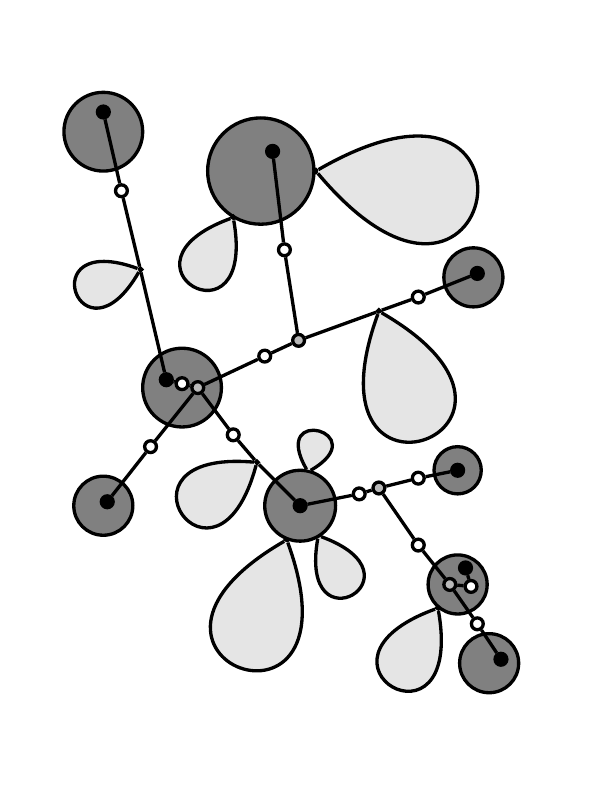
\begin{tikzpicture}[every node/.style={draw, very thick}, every path/.style={very thick}]
    
    \node[circle, draw, minimum size = 1cm, fill=gray] (1) at (-3,2.75) {};
    \node[circle, draw, minimum size=0.15cm, inner sep=0pt, fill=black] (2) at (-3,3) {};

    
    
    \node[circle, draw, minimum size = 1.35cm, fill=gray] (3) at (-1,2.25) {};
    \node[circle, draw, minimum size=0.15cm, inner sep=0pt, fill=black] (4) at (-0.85,2.5) {};
    \node[circle, draw, inner sep=0pt, fill=white] (36) at (-0.3,2.25) {};
    \node[circle, draw, inner sep=0pt, fill=white] (40) at (-1.35,1.66) {};
    

    
    \node[circle, draw, minimum size=0.15cm, inner sep=0pt, fill=white] (5) at (-2.77,2) {};
    
    \node[circle, draw, minimum size=0.15cm, inner sep=0pt, fill=white] (6) at (-0.7,1.25) {};
    
    \node[circle, draw, minimum size = 0.75cm, fill=gray] (7) at (1.7,0.9) {};
    \node[circle, draw, minimum size=0.15cm, inner sep=0pt, fill=black] (8) at (1.75,0.95) {};
    
    \node[circle, draw, inner sep=0pt, fill=white] (9) at (-2.53,1) {};
    
    \node[circle, draw, minimum size=0.15cm, inner sep=0pt, fill=white] (10) at (1,0.65) {};
    
    \node[circle, draw, inner sep=0pt, fill=white] (11) at (0.5,0.47) {};
    
    \node[circle, draw, minimum size=0.15cm, inner sep=0pt, fill=gray!55] (12) at (-0.52,0.1) {};
    
    \node[circle, draw, minimum size=0.15cm, inner sep=0pt, fill=white] (13) at (-0.95,-0.1) {};

    
    \node[circle, draw, minimum size = 1cm, fill=gray] (14) at (-2,-0.5) {};
    \node[circle, draw, minimum size=0.15cm, inner sep=0pt, fill=black] (15) at (-2.2,-0.4) {};
    \node[circle, draw, minimum size=0.15cm, inner sep=0pt, fill=white] (16) at (-2,-0.45) {};
    \node[circle, draw, minimum size=0.15cm, inner sep=0pt, fill=gray!55] (17) at (-1.8,-0.5) {};
    
    \node[circle, draw, minimum size=0.15cm, inner sep=0pt, fill=white] (18) at (-1.35,-1.1) {};

    \node[circle, draw, minimum size=0.15cm, inner sep=0pt, fill=white] (19) at (-2.4,-1.25) {};
    
    \node[circle, draw, inner sep=0pt, fill=white] (20) at (-1.05,-1.45) {};
    
    \node[circle, draw, minimum size = 0.6cm, fill=gray] (21) at (1.5,-1.55) {};
    \node[circle, draw, minimum size=0.15cm, inner sep=0pt, fill=black] (22) at (1.5,-1.55) {};
    
    \node[circle, draw, minimum size=0.15cm, inner sep=0pt, fill=white] (23) at (1,-1.65) {};
    
    \node[circle, draw, minimum size=0.15cm, inner sep=0pt, fill=gray!55] (24) at (0.5,-1.775) {};
    
    \node[circle, draw, minimum size=0.15cm, inner sep=0pt, fill=white] (25) at (0.25,-1.85) {};

    \node[circle, draw, minimum size = 0.75cm, fill=gray] (26) at (-3,-2) {};
    \node[circle, draw, minimum size=0.15cm, inner sep=0pt, fill=black] (27) at (-2.95,-1.95) {};
    \node[circle, draw, inner sep=0pt, fill=white] (41) at (-0.67,-2.433) {};
    \node[circle, draw, inner sep=0pt, fill=white] (42) at (-0.27,-2.38) {};
    \node[circle, draw, inner sep=0pt, fill=white] (43) at (-0.4,-1.57) {};
    
    \node[circle, draw, minimum size = 0.9cm, fill=gray] (28) at (-0.5,-2) {};
    \node[circle, draw, minimum size=0.15cm, inner sep=0pt, fill=black] (29) at (-0.5,-2) {};

    
    \node[circle, draw, minimum size=0.15cm, inner sep=0pt, fill=white] (30) at (1,-2.5) {};
    
    \node[circle, draw, minimum size = 0.75cm, fill=gray] (31) at (1.5,-3) {};
    \node[circle, draw, minimum size=0.15cm, inner sep=0pt, fill=gray!55] (32) at (1.4,-3) {};
    \node[circle, draw, inner sep=0pt, fill=white] (37) at (1.25,-3.3) {};
    \node[circle, draw, minimum size=0.15cm, inner sep=0pt, fill=black] (38) at (1.6,-2.79) {};
    \node[circle, draw, minimum size=0.15cm, inner sep=0pt, fill=white] (39) at (1.67,-3.025) {};
    
    \node[circle, draw, minimum size=0.15cm, inner sep=0pt, fill=white] (33) at (1.75,-3.5) {};
    
    \node[circle, draw, minimum size = 0.75cm, fill=gray] (34) at (1.9,-4) {};
    \node[circle, draw, minimum size=0.15cm, inner sep=0pt, fill=black] (35) at (2.05,-3.95) {};
    
    \draw[] (2) to (5);
    \draw[] (4) to (6);
    \draw[] (5) to (9);
    \draw[] (6) to (12);
    \draw[] (8) to (10);
    \draw[] (9) to (15);
    \draw[] (10) to (11);
    \draw[] (11) to (12);
    \draw[] (12) to (13);
    \draw[] (13) to (17);
    \draw[] (15) to (16);
    \draw[] (16) to (17);
    \draw[] (17) to (18);
    \draw[] (17) to (19);
    \draw[] (18) to (20);
    \draw[] (19) to (27);
    \draw[] (20) to (29);
    \draw[] (22) to (23);
    \draw[] (23) to (24);
    \draw[] (24) to (25);
    \draw[] (24) to (30);
    \draw[] (25) to (29);
    \draw[] (30) to (32);
    \draw[] (32) to (33);
    \draw[] (32) to (39);
    \draw[] (33) to (35);
    \draw[] (38) to (39);
    \draw[very thick, fill=gray!20]
    (9).. controls +(-120:1.5cm) and +(-200:1.5cm).. (9);
    \draw[very thick, fill=gray!20]
    (11).. controls +(-30:3cm) and +(-110:3cm).. (11);
    \draw[very thick, fill=gray!20]
    (20).. controls +(-105:2cm) and +(-185:2cm).. (20);
    \draw[very thick, fill=gray!20]
    (36).. controls +(30:3.6cm) and +(-50:3.6cm).. (36);
    \draw[very thick, fill=gray!20]
    (37).. controls +(-80:2cm) and +(-160:2cm).. (37);
    \draw[very thick, fill=gray!20]
    (40).. controls +(-80:1.75cm) and +(-160:1.75cm).. (40);
    \draw[very thick, fill=gray!20]
    (41).. controls +(-70:3cm) and +(-150:3cm).. (41);
    \draw[very thick, fill=gray!20]
    (42).. controls +(-20:1.5cm) and +(-100:1.5cm).. (42);
    \draw[very thick, fill=gray!20]
    (43).. controls +(120:1cm) and +(30:1cm).. (43);
    
    \end{tikzpicture}
    \caption{Example tree $\mathcal{T}$. Dark grey circles represent heavy modules. Light grey regions represent light subtrees. Black vertices represent $\mathcal{X}$. Gray and black vertices represent $\mathcal{Y}$. White, gray and black vertices represent $\mathcal{Z}$. Lines represent paths of vertices between vertices of $\mathcal{Z}$.}\label{exampleTreeWithSetZ}
\end{minipage}
    \hspace{0.06\textwidth} % Add space between the two minipages
    \begin{minipage}[t]{0.47\textwidth}
    \centering
    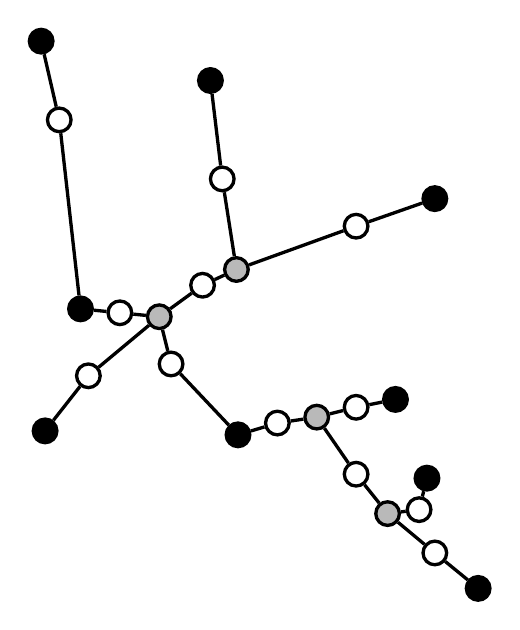
\begin{tikzpicture}[every node/.style={draw, very thick}, every path/.style={very thick}]
    
    \node[circle, draw, minimum size=0.3cm, inner sep=0pt, fill=black] (2) at (-3,4) {};

    
    
    \node[circle, draw, minimum size=0.3cm, inner sep=0pt, fill=black] (4) at (-0.85,3.5) {};
    

    
    \node[circle, draw, minimum size=0.3cm, inner sep=0pt, fill=white] (5) at (-2.77,3) {};
    
    \node[circle, draw, minimum size=0.3cm, inner sep=0pt, fill=white] (6) at (-0.7,2.25) {};
    
    \node[circle, draw, minimum size=0.3cm, inner sep=0pt, fill=black] (8) at (2,2) {};
    
    
    \node[circle, draw, minimum size=0.3cm, inner sep=0pt, fill=white] (10) at (1,1.65) {};
    
    
    \node[circle, draw, minimum size=0.3cm, inner sep=0pt, fill=gray!55] (12) at (-0.52,1.1) {};
    
    \node[circle, draw, minimum size=0.3cm, inner sep=0pt, fill=white] (13) at (-0.95,0.9) {};

    
    \node[circle, draw, minimum size=0.3cm, inner sep=0pt, fill=black] (15) at (-2.5,0.6) {};
    \node[circle, draw, minimum size=0.3cm, inner sep=0pt, fill=white] (16) at (-2,0.55) {};
    \node[circle, draw, minimum size=0.3cm, inner sep=0pt, fill=gray!55] (17) at (-1.5,0.5) {};
    
    \node[circle, draw, minimum size=0.3cm, inner sep=0pt, fill=white] (18) at (-1.35,-0.1) {};

    \node[circle, draw, minimum size=0.3cm, inner sep=0pt, fill=white] (19) at (-2.4,-0.25) {};
    
    
    \node[circle, draw, minimum size=0.3cm, inner sep=0pt, fill=black] (22) at (1.5,-0.55) {};
    
    \node[circle, draw, minimum size=0.3cm, inner sep=0pt, fill=white] (23) at (1,-0.65) {};
    
    \node[circle, draw, minimum size=0.3cm, inner sep=0pt, fill=gray!55] (24) at (0.5,-0.775) {};
    
    \node[circle, draw, minimum size=0.3cm, inner sep=0pt, fill=white] (25) at (0,-0.85) {};

    \node[circle, draw, minimum size=0.3cm, inner sep=0pt, fill=black] (27) at (-2.95,-0.95) {};
    
    \node[circle, draw, minimum size=0.3cm, inner sep=0pt, fill=black] (29) at (-0.5,-1) {};

    
    \node[circle, draw, minimum size=0.3cm, inner sep=0pt, fill=white] (30) at (1,-1.5) {};
    
    \node[circle, draw, minimum size=0.3cm, inner sep=0pt, fill=gray!55] (32) at (1.4,-2) {};
    \node[circle, draw, minimum size=0.3cm, inner sep=0pt, fill=black] (38) at (1.9,-1.55) {};
    \node[circle, draw, minimum size=0.3cm, inner sep=0pt, fill=white] (39) at (1.8,-1.95) {};
    
    \node[circle, draw, minimum size=0.3cm, inner sep=0pt, fill=white] (33) at (2,-2.5) {};
    
    \node[circle, draw, minimum size=0.3cm, inner sep=0pt, fill=black] (35) at (2.55,-2.95) {};
    
    \draw[] (2) to (5);
    \draw[] (4) to (6);
    \draw[] (5) to (15);
    \draw[] (6) to (12);
    \draw[] (8) to (10);
    \draw[] (10) to (12);
    \draw[] (12) to (13);
    \draw[] (13) to (17);
    \draw[] (15) to (16);
    \draw[] (16) to (17);
    \draw[] (17) to (18);
    \draw[] (17) to (19);
    \draw[] (18) to (29);
    \draw[] (19) to (27);
    \draw[] (22) to (23);
    \draw[] (23) to (24);
    \draw[] (24) to (25);
    \draw[] (24) to (30);
    \draw[] (25) to (29);
    \draw[] (30) to (32);
    \draw[] (32) to (33);
    \draw[] (32) to (39);
    \draw[] (33) to (35);
    \draw[] (38) to (39);
    \end{tikzpicture}
    \caption{Auxiliary tree $\mathcal{T}_{\mathcal{Z}}$ built from vertices of set $\mathcal{Z}$. Lines represent edges between vertices of $\mathcal{T}_{\mathcal{Z}}$.}\label{exampleAuxTreeTZ}
\end{minipage}
\end{figure}
\begin{lemma}\label{auxTreeCostLemma}
    Let $\mathcal{T}_{\mathcal{Z}}$ be the auxiliary tree. Then, $\OPT\br{\mathcal{T}_{\mathcal{Z}}}\leq \OPT\br{\mathcal{T}}$.
    \begin{proof}
        Let $D^*$ be the optimal strategy for $\mathcal{T}\angl{\mathcal{Z}}$. We build a new decision tree $D_{\mathcal{Z}}'$ for $\mathcal{T}_{\mathcal{Z}}$ by transforming $D^*$: Let $u,v\in \mathcal{Y}$ such that $\mathcal{P}_{\mathcal{T}}\br{u, v}\neq\emptyset$ and $\mathcal{P}_{\mathcal{T}}\br{u, v}\cap \mathcal{Y}=\emptyset$. Let $q\in V\br{D^*}$ such that $q\in \mathcal{P}_{\mathcal{T}}\br{u, v}$ is the first query among vertices of $\mathcal{P}_{\mathcal{T}}\br{u, v}$. We replace $q$ in $D^*$ by the query to the distinct vertex $v_{u,v}\in \mathcal{P}_{\mathcal{T}}\br{u, v}\cap \mathcal{Z}$ and delete all queries to vertices $\mathcal{P}_{\mathcal{T}}\br{u, v}-v_{u,v}$ from $D^*$. By construction, $D_{\mathcal{Z}}'$ is a valid decision tree for $\mathcal{T}_{\mathcal{Z}}$ and as for every $z\in \mathcal{P}_{\mathcal{T}}\br{u, v}$: $c\br{v_{u,v}}\leq c\br{z}$ such strategy has cost at most $\COST_{D_{\mathcal{Z}}'}\br{\mathcal{T}_{\mathcal{Z}}}\leq \OPT\br{\mathcal{T}\angl{\mathcal{Z}}}$. We get:
        $$
        \OPT\br{\mathcal{T}_{\mathcal{Z}}}\leq \COST_{D_{\mathcal{Z}}'}\br{\mathcal{T}_{\mathcal{Z}}}\leq \OPT\br{\mathcal{T}\angl{\mathcal{Z}}}\leq \OPT\br{\mathcal{T}}
        $$

        where the first inequality is due to the optimality and the last inequality is due to the fact that $\mathcal{T}\angl{\mathcal{Z}}$ is a subtree of $\mathcal{T}$ (by Lemma \ref{lemma:subtreeCost}). The lemma follows.
    \end{proof}
\end{lemma}

\begin{lemma}
    $\COST_D\br{\mathcal{T}}\leq\COST_{D_C}\br{\mathcal{T}_C}+\br{2+\frac{b}{a}}\OPT\br{\mathcal{T}}$
    \begin{proof}
    Let $H\subseteq V\br{\mathcal{T}}$ be a heavy module. We show that: $\COST_{D_H}\br{\mathcal{T}\angl{H}}\leq \frac{b}{a}\cdot\OPT\br{\mathcal{T}, c}$. For every $v\in H$ let $c'\br{v}=a$ (note, that we can choose any cost here since we treat each query as unitary). As $\frac{bc'\br{v}}{a}\geq b \geq c\br{v}$ we get that $\frac{b}{a}\cdot\COST_{D_H}\br{\mathcal{T}\angl{H}, c'}\geq \COST_{D_H}\br{\mathcal{T}\angl{H}, c}$. Additionally, using the fact that $c'\br{v} \leq c\br{v}$ we get that $\OPT\br{\mathcal{T}\angl{H}, c'}\leq \OPT\br{\mathcal{T}\angl{H}, c}$. Therefore:
    $$
    \begin{gathered}
        \COST_{D_H}\br{\mathcal{T}\angl{H}, c}\leq \frac{b}{a}\cdot\COST_{D_H}\br{\mathcal{T}\angl{H}, c'}=\frac{b}{a}\cdot\OPT\br{\mathcal{T}\angl{H}, c'}\leq \\
        \leq
        \frac{b}{a}\cdot\OPT\br{\mathcal{T}\angl{H}, c}\leq \frac{b}{a}\cdot\OPT\br{\mathcal{T}, c}
    \end{gathered}
    $$
        
    where the last inequality is due to the fact that $\mathcal{T}\angl{H}$ is a subtree of $\mathcal{T}$ (by Lemma \ref{subtreeCostLemma}).
        
    Let $Q_D\br{\mathcal{T},x}$ be a sequence of queries performed in order to find target $x$. By construction of the Algorithm \ref{extensionProcedure}, $Q_D\br{\mathcal{T},x}$ consists of at most three distinct subsequences of queries (some subsequences might be empty). Firstly, there is a sequence of queries belonging to $Q_{D_{\mathcal{Z}}}\br{\mathcal{T}_{\mathcal{Z}},x}$. If $x\notin \mathcal{Z}$, then it is followed by a sequence of queries belonging to $Q_{D_{H}}\br{\mathcal{T}\angl{H},x}$ such that $H\in \mathcal{T}'$ is a heavy module and $x\in \mathcal{T}'$. If $x\notin H$, at last, there is a sequence of queries belonging to $Q_{D_{L}}\br{L,x}$ for $L\in \mathcal{T}'-H$ such that $x\in L$. 
    We have:
        \begin{align*}
        \COST_D\br{\mathcal{T}}&\leq
        \COST_{D_{\mathcal{Z}}}\br{\mathcal{T}}+\max_{\mathcal{T}'\in \mathcal{T}-\mathcal{Z}}\brc{\COST_{D_H}\br{\mathcal{T}\angl{H}}+\max_{L\in \mathcal{T}'-H}\brc{\COST_{D_L}\br{L}}}
        \\ 
        &\leq
        \COST_{D_{\mathcal{Z}}}\br{\mathcal{T}_{\mathcal{Z}}}+\max_{\mathcal{T}'\in \mathcal{T}-\mathcal{Z}}\brc{\frac{b}{a}\cdot\OPT\br{\mathcal{T}}+\COST_{D_C}\br{\mathcal{T}_C}}
        \\
        &\leq
        2\OPT\br{\mathcal{T}_{\mathcal{Z}}}+\frac{b}{a}\cdot\OPT\br{\mathcal{T}}+ \COST_{D_C}\br{\mathcal{T}_C} \leq \COST_{D_C}\br{\mathcal{T}_C} + \br{2+\frac{b}{a}}\cdot\OPT\br{\mathcal{T}}
        \end{align*}

        where the first inequality is due to the construction of the returned decision tree, the second is due to Observation \ref{CostDZinTObservation} and due to the fact that $L$ is a subtree of $\mathcal{T}_C$ (Lemma \ref{lemma:subtreeCost}), the third is due is due to Theorem \ref{QPTAS} and the last is due to Lemma \ref{auxTreeCostLemma}.
        
    \end{proof}
\end{lemma}

Using Lemma \ref{auxTreeSizeLemma} we get that the QPTAS runs in time $2^{O\br{\log^2\br{4k\br{\mathcal{T}}}}}=2^{O\br{\log^2\br{k\br{\mathcal{T}}}}}$ and all other computations can be performed in polynomial time which completes the proof of the Proposition \ref{existanceOfExtensionAlgorithm}.

\subsection{Average case, non-uniform weights}
In this section we show how to obtain a constant factor approximation for the $T||V,c,w||\sum C_i$ problem. Since the problem is NP-hard, one should not hope for a polynomial time exact solution (The proof of this fact is differed to the appendix). However, even constant factor approximation is quite surprising as in contrast, recall that the state-of-the-art algorithm for $T||V,c||C_{max}$ achieves only much weaker, $O\br{\sqrt{\log n}}$-approximation. The idea behind the solution is inspired by the work of \cite{Approximatehierarchicalclusteringviasparsestcutandspreadingmetrics} and \cite{kseparator}. In order to tightly lower bound the cost of the optimum we use the connection of the problem to the following weighted $\alpha$-separator problem which is a generalization of the $k$-separator problem introduced in \cite{kseparator}:
\paragraph{Weighted $\alpha$-separator problem}
\begin{tcolorbox}[colback=white, title=Weighted $\alpha$-separator problem, fonttitle=\bfseries, breakable]
\paragraph{Input:} Graph $G=\br{V\br{G}, E\br{G}}$, the weight function $w:V\to \mathbb{N}^+$, the cost function $c:V\to \mathbb{N}^+$ and a real number $\alpha$.
\paragraph{Output:} A set $S\subseteq V\br{G}$ called \textit{separator} such that for every $H\in G-S$: $w\br{S}\leq w\br{G}/\alpha$ and $c\br{S}$ is minimized.
\end{tcolorbox}

Note that the authors of \cite{kseparator} use an alternative definition for the unweighted version of the problem in which the size of each $H\in G-S$ is required to be $\spr{H}\leq k$. As we are concerned with the more general variant of the problem it is easier for us to use our definition. Given the value $\alpha$ or $k$ one can obtain the other by simply using the fact that the problems are equivalent when $k=w\br{G}/\alpha$. We will use these two notions whenever more comfortable. Note that for the special case when $\alpha=0$ we have that $k=\infty$ and the optimal separator for $G$ is $\emptyset$.

For the sake of our analysis we will be only concerned with the variant in which the underlying graph is a tree. When the weights are uniform, this problem is solvable in polynomial time \cite{kseparator}. 
If otherwise, the problem is (weakly) NP-hard. The proof of this fact is differed to the appendix. Despite the hardness of the problem we show that it can be solved in a pseudopolynomial time by means of dynamic programming.


\begin{theorem}
    There exists a $O\br{n\br{\min\brc{c\br{T}, w\br{T}/\alpha}}^2}$ time algorithm for the Weighted $\alpha$-separator Problem.
    \begin{proof}
        We use separate subprocedures depending on which of the values $c\br{T}, w\br{T}$ is smaller. Both of them are inspired by the polynomial time algorithm for the unweighted version of the problem \cite{kseparator}. We assume that that the input tree is rooted in an arbitrary vertex $r$. For any vertex $v\in V\br{T}$ let $\mathcal{C}_T\br{v}=\brc{c_1,c_2,\dots,c_{\deg_v^+}}$.
        \begin{enumerate}
            \item $w\br{T}/\alpha\leq c\br{T}$. Let $C_{v}$ be the cost of the optimal separator of the subtree $T_v$. Define $C_{v}^{in}$ as the cost of the optimal $\alpha$-separator $S$ under the condition that $v$ belongs to $S$. We immediately have the following relationship:
            $$
            C_{v}^{in} = c\br{v}+\sum_{c\in \mathcal{C}\br{v}}C_{c}
            $$
            Assume that $v\notin S$. Let $H^v\in T-S$ such that $v\in H^v$. For each $1\leq w\leq k$ let $C_v^{out}\br{w}$ denote the cost of the optimal $\alpha$-separator $S$ such that $v\notin S$ and $w\br{H^v} = w$. We have that:
            $$
            C_v = \min\brc{C_{v}^{in},\min_{1\leq w\leq k}C_v^{out}\br{w}}
            $$
            
            For any vertex $v\in V\br{T}$ and any number $1\leq i\leq \deg_v^+$ let $H_{v,i}\in T_{v,i}-S$ such that $v\in H_{v,i}$. Additionally, for any number $1\leq w\leq k$ let $C_{v,i}^{out}\br{w}$ denote the weight of an optimal $\alpha$-separator such that $v\notin S$ and $w\br{H_i^v} = w$. We have that: 
            $$
            C_{v}^{out}\br{w}=C_{v,\deg_v^+}^{out}\br{w}
            $$
            $$
            C_{v,1}^{out}\br{w}=\begin{cases}
                \infty, & \text{if } w < w\br{v}\\
                C_{c_1}^{in}, & \text{if } w = w\br{v}\\
                C_{c_1}^{out}\br{w-w\br{v}}, & \text{if } w > w\br{v}\\
            \end{cases}
            $$
            $$
            C_{v,i}^{out}\br{w}=\min\brc{C_{v,i-1}^{out}\br{w}+C_{c_i}^{in}, \min_{1\leq j\leq w-1}\brc{C_{v,i-1}^{out}\br{w-j}+C_{c_i}^{out}\br{j}}}
            $$
            Where in the last equality the  first term of the minimum function represents a situation in which $c_i\in S$. In such case all of the weight of $H_{v, i}$ belongs to $H_{i-1}^v$. The second term assumes contrary and checks all possible partitions of the weight between $T_{v, i-1}$ and $T_{c_i}$.

            The relationships above suffice to calculate the value of $C_{r}$ which is the cost of the optimal separator $S$. The computation is performed in a bottom-up, left to right manner starting with the leafs. To finish the description of the algorithm we observe then when this is the case ($v$ is a leaf) we have that $C_v^{in}=c\br{v}$, $C_v^{out}\br{w}=0$, $C_v = 0$ and all other values are equal to $\infty$.

            As there are $O\br{nw\br{T}/\alpha}$ subproblems and each of them requires at most $w\br{T}/\alpha$ computational steps we obtain that the running time is  $O\br{n\br{w\br{T}/\alpha}^2}$.
            \item $w\br{T}/\alpha\geq c\br{T}$. For $v\in V\br{T}$ and $1\leq c\leq c\br{T}$ let $W_{v}\br{c}$ be the optimal weight of $H_v$ in the separator of the subtree $T_v$ of cost at most $c$. Let $B\br{v, c}$ be a boolean value defined as:
            $$
            B_{v}\br{c}=\begin{cases}
                0, & \text{if } W_{v}\br{c} \leq k\\
                1, & \text{if } W_{v}\br{c} > k\\
            \end{cases}
            $$
            Define a boolean value $B_{v}^{in}\br{c}$ to be $0$: if there exists a separator of the subtree $T_v$ of cost at most $c$ under the condition that $v$ belongs to $S$ and $1$ if otherwise. For $1\leq i\leq \deg_{v}^+$ we also define a boolean value $B_{v, i}^{in}\br{c}$ to be $0$: if there exists a separator of the subtree $T_{v,i}$ of cost at most $c$ under the condition that $v$ belongs to $S$ and $1$ if otherwise. Of course $B_{v}^{in}\br{c}=B_{v, \deg_v^+}^{in}\br{c}$. We have the following relationships:
            $$
            B_{v,1}^{in}\br{c}=\begin{cases}
                1, & \text{if } c < c\br{v}\\
                B_{c_1}\br{c-c\br{v}}, & \text{if } c \geq c\br{v}\\
            \end{cases}
            $$
            $$
            B_{v, i}^{in}\br{c} = \min_{1\leq j\leq c}\brc{B_{v, i-1}^{in}\br{c-j}\lor B_{c_i}\br{j}}
            $$
            For each $1\leq c\leq c\br{T}$ let $W_v^{out}\br{w}$ denote the optimal weight of $H^v$ in the separator of the subtree $T_v$ of cost at most $c$ under assumption that $v\notin S$. We have that:
            $$
            W_v\br{c} = \begin{cases}
                0, & \text{if } \neg B_{v}^{in}\br{c}\\
                W_v^{out}\br{c}, & \text{otherwise }
            \end{cases}
            $$
            
            For any vertex $v\in V\br{T}$ and for any number $1\leq c\leq c\br{T}$ let $W_{v,i}^{out}\br{c}$ denote the optimal weight of $H_i^v$ in the separator of the subtree $T_{v,i}$ of cost at most $c$ under assumption that $v\notin S$. We have that: 
            $$
            W_{v}^{out}\br{c}=W_{v,\deg_v^+}^{out}\br{c}
            $$ 
            If $v$ has only one child we have that:
            $$
            W_{v,1}^{out}\br{c}=\begin{cases}
                \infty, & \text{if } B_{c_1}^{in}\br{c}\\
                w\br{v} + W_{c_1}\br{c}, & \text{otherwise } \\
            \end{cases}
            $$
            It is also easy to see that for $i>1$ we have:
            $$
            W_{v,i}^{out}\br{c}=\min_{1\leq j\leq c}\brc{W_{v,i-1}^{out}\br{c-j}+W_{c_i}\br{j}}
            $$
            
            To obtain the cost of the optimal separator we calculate the value $\min\brc{1\leq c \leq c\br{T} | B_{r}\br{c}=0}$ which is the minimal value for which a valid separator of cost at most $c$ exists. The computation is performed in a bottom-up, left to right manner starting with the leafs. To finish the description of the algorithm we observe then when this is the case ($v$ is a leaf) we have that: 
            $$
            B_v^{in}\br{c}=\begin{cases}
                0, & \text{if } c=c\br{v}\\
                1, & \text{otherwise }\\
            \end{cases}$$
            And also:
            $$
            W_v^{out}\br{c}=\begin{cases}
                w\br{v}, & \text{if } c=0\\
                \infty, & \text{otherwise }\\
                \end{cases}
            $$

            As there are $O\br{nc\br{T}}$ subproblems and each of them requires at most $c\br{T}$ computational steps we obtain that the running time is  $O\br{nc\br{T}^2}$.
        \end{enumerate}
        
         To obtain not only the value of the optimum but also a solution, in both cases, by using a standard tabling one is able to store the information about the vertices belonging to the optimal separator for all calculated subproblems.
    \end{proof}
\end{theorem}
    We would like to use the previously shown procedure the create a constant-factor approximation algorithm for $T||V,c,w||\sum C_i$. However, the running time of this algorithm may not be polynomial if both $c\br{T}$ and $w\br{T}$ are of order $\omega\br{\text{poly}\br{n}}$. To alleviate this difficulty we will use a fairly standard rounding trick which will provide us with  a bi-criteria FPTAS for the weighted $\alpha$-separator.
    
    Let $\OPT_\alpha$ be the cost of the optimal solution for the chosen value of $\alpha$. We will still require that the cost of the returned solution will be at most $\OPT_\alpha$. However, we will relax the condition demanding that $H\in T-S$: $w\br{H}\leq \frac{w\br{T}}{\alpha}$ and we will only require that $w\br{H}\leq \frac{\br{1+\delta}w\br{T}}{\alpha}$ for some chosen value of $\delta$. 
\begin{theorem}
    Let $S^*$ be an optimal weighted $\alpha$-separator for $\br{T,c,w,\alpha}$. For any $\delta>0$ there exists an algorithm which returns a separator $S$ such that:
    \begin{enumerate}
        \item $w\br{H}\leq \frac{\br{1+\delta}\cdot w\br{T}}{\alpha}$ for every $H\in T-S$.
        \item $c\br{S}\leq c\br{S^*}$.
    \end{enumerate}
    The algorithm runs in $O\br{n^3/\delta^2}$ time.
    \begin{proof}
        The procedure is as follows:
        \begin{enumerate}
            \item Let $K=\frac{\delta W}{n\alpha}$, for every $v\in V\br{T}$: $w'\br{v} = \fl{\frac{w\br{v}}{K}}$, $w'\br{T}=\sum_{v\in V\br{T}}w'\br{v}$ and $\alpha'=\frac{w'\br{T}K\alpha}{w\br
            T}$.
            \item Return the optimal separator $S$ for $\br{T, w', c, \alpha'}$ found using the $O\br{n\br{\frac{W}{\alpha}}^2}$ time algorithm.
        \end{enumerate}
        \begin{lemma}
            Let $S^*$ be the optimal separator for the original instance. $C\br{S}\leq C\br{S^*}$.
            \begin{proof}
                We prove that $S^*$ is a valid separator for the $\br{T, w', c, \alpha'}$ instance. 
                Recall that $k=W\br{T}/\alpha$.
                To simplify the analysis we introduce the auxiliary instance with values: $$
                w''\br{v} = \fl{\frac{w\br{v}}{K}}\cdot K, 
                w''\br{T}=\sum_{v\in V\br{T}}w''\br{v}, k'' = k \text{ and consequently: } \alpha'' = \frac{w''\br{T}}{k''}=\frac{\alpha w''\br{T}}{w\br{T}}$$
                
                Notice that in this new instance the absolute threshold for required size of each $H \in T-S^*$ has not changed ($k'' = k$) and for every $v\in V\br{T}$: $w''\br{v}\leq w\br{v}$.  Therefore we have that $w''\br{H}\leq w\br{H}\leq k\leq \frac{w''\br{T}}{\alpha''}$. Now notice that the one prim instance has all of its weights scaled by a constant value of $K$ and the relative factor of $\alpha' = \alpha''$. As multiplying by a constant does not influence the validity of a solution $S^*$ is a valid $\alpha'$-separator for $\br{T, w', c, \alpha'}$. Additionally, as the costs remained unchanged and $S$ is optimal for $\br{T, w', c, \alpha'}$ the claim follows.
            \end{proof}
        \end{lemma}
        \begin{lemma}
            For every $H\in T-S$ we have that $w\br{H}\leq\frac{\br{1+\delta}w\br{T}}{\alpha}$.
            \begin{proof}
                By definition we have that $w'\br{v}\leq \frac{w\br{v}}{K}\leq w'\br{v}+1$ and therefore also $Kw'\br{v}\leq w\br{v}\leq Kw'\br{v}+K$. We have that:
                $$
                \sum_{v\in H}w\br{v}\leq K\cdot\sum_{v\in H}w'\br{v}+Kn\leq \frac{Kw'\br{T}}{\alpha'}+nK = \frac{w\br{T}}{\alpha} + \frac{\delta w\br{T}}{\alpha}=\frac{\br{1+\delta}w\br{T}}{\alpha}
                $$
                
                where the second inequality is due to the fact that $S$ is a $\alpha'$-separator for $\br{T, w'\br{T}, c, \alpha'}$ instance.
            \end{proof}
        \end{lemma}
        
        Combining the two above lemmas with the fact that $\frac{w'\br{T}}{\alpha'}=\frac{w\br{T}}{K\alpha}=\frac{n}{\delta}$ we have that the algorithm runs in time $O\br{n^3/\delta^2}$ as required.
    \end{proof}
\end{theorem}
\paragraph{Constant-factor approximation for $T||V, w, c||\sum C_i$}
    As it turns out the $T||V, w, c||\sum C_i$ is deeply connected with the previously regarded Separator Problem. The idea behind the construction and the analysis of the algorithm is largely inspired by \cite{Approximatehierarchicalclusteringviasparsestcutandspreadingmetrics}. In order to tightly lower bound the value of the optimal solution, we split the cost of the optimal solution into levels, one for each $0\leq k < w\br
    T$, such that each level consists of a $w\br{T}/k$-separator of $T$.
    
    We start with some additional notation. By $L_{\OPT}\br{k}$ we will denote the set of all maximal subtrees of weight at most $k$ in $\OPT$. We call such set the $k$-th \textit{level} of $\OPT$. Observe that as two candidate subtrees $H_1, H_2$ may only have a common part when $H_1\subseteq H_2$ or $H_2\subseteq H_1$, by the minimality we have that $H_1 \cap H_2 =\emptyset$. We denote $S_{\OPT}\br{k}=V\br{T}-L_{\OPT}\br{k}$. These are the vertices belonging to the separator at the level $L_{\OPT}\br{k}$. 
    
            \begin{lemma}
                $\OPT=\sum_{k=0}^{w\br{T}-1}c\br{S_{\OPT}\br{k}}$
            \begin{proof}
                Consider any vertex $v$ and let $r$ be the weight of the subtree of candidates right before $v$ is queried. Then the contribution of $v$ to the LHS is $r\cdot c\br{v}$. On the other hand, for every $0\leq k<r$ we have that $v\in S_{\OPT}\br{k}$ so the contribution to the RHS is $r\cdot c\br{v}$ as well.
            \end{proof}
            \end{lemma}
            Using the above lemma one easily obtains the following lower bound on the cost of the optimal solution:
            $$
            2\cdot\OPT= 2\cdot\sum_{k=0}^{w\br{T}-1}c\br{S_{\OPT}\br{k}} \geq \sum_{k=0}^{w\br{T}}c\br{S_{\OPT}\br{\fl{k/2}}}
            $$
             
    Using the above lower bound on the value of $\OPT$ we will prove the main result of this section, namely:
    \begin{theorem}
        There exists a $4$-approximation algorithm for $T||V, w, c||\sum C_i$ running in time $O\br{n^2\br{\min\brc{c\br{T}, w\br{T}/\alpha}}^2}$ and a $\br{4+\epsilon}$-approximation algorithm running in time $O\br{n^4/\epsilon^2}$.
        \begin{proof}
            We describe how the obtain the $\br{4+\epsilon}$-approximation since the pseudopolynomial time algorithm can be formulated and analyzed similarly (using the exact algorithm for the weighted separator problem with $\alpha=2$).
            The procedure is as follows: 
            
\begin{algorithm}[H]
\caption{The $\br{4+\epsilon}$-approximation algorithm for $T||V,c,w||\sum{C_i}$.}
\label{createDecisionTree}
\SetKwFunction{FDecisionTree}{DecisionTree}
\SetKwFunction{FSeparatorFPTAS}{SeparatorFPTAS}
\SetKwProg{Fn}{Procedure}{:}{}
\Fn{\FDecisionTree{$T, c, w,  \epsilon$}}{
$S_T\gets$ \FSeparatorFPTAS$\br{T, c, w, \alpha=2, \delta = \frac{\epsilon}{4+\epsilon}}$

Build an arbitrary decision tree $D_T$ on vertices of $S_T$.

    \ForEach{$H\in T-S$}
    {
        $D_H\gets $\FDecisionTree{$H, c, w, \epsilon$}

        Hang $D_H$ below the last query consistent with $H$ in $D_T$.
    }   
    \Return $D$
    
}
\end{algorithm}
            \begin{figure}[htbp]
    \centering
    \begin{minipage}{0.48\textwidth}
    \centering
        \begin{tikzpicture}[scale=0.95]
    \draw[thick, fill=white, drop shadow]
  (0,0) 
  .. controls (1,0) and (1,-6) .. (0,-6)  % right side curve
  .. controls (-1,-6) and (-1,0) .. (0,0); % left side curve
  
  \node at (-0.75, 0)  {$S_T$};

Dots inside
\foreach \y in {-1,-2,-3,-5} {
  \fill (0,\y) circle (4pt);
}
\node at (0, -3.9) {$\vdots$};

\draw[thick, fill=white, drop shadow]
(3,0.75) 
  .. controls (4.5,0.75) and (4.5,-0.75) .. (3,-0.75)  % right side curve
  .. controls (1.5,-0.75) and (1.5,0.75) .. (3,0.75); % left side curve

\node at (3, -0.05)  {$H_1$};

\draw[thick] (0.45,-0.5) -- (1.87,0);

\draw[thick] (0.745,-2.5) -- (2.04,-0.4);

\draw[thick, fill=white, drop shadow]
(3.5,-1) 
  .. controls (4.5,-1) and (4.5,-2) .. (3.5,-2)  % right side curve
  .. controls (2.5,-2) and (2.5,-1) .. (3.5,-1); % left side curve

\node at (3.5, -1.55)  {$H_2$};

\draw[thick] (0.66,-1.6) -- (2.74,-1.5);

\draw[thick, fill=white, drop shadow]
(3.25,-2.25) 
  .. controls (4.5,-2.25) and (4.5,-3.5) .. (3.25,-3.5)  % right side curve
  .. controls (2,-3.5) and (2,-2.25) .. (3.25,-2.25); % left side curve

\node at (3.25, -2.9)  {$H_3$};

\draw[thick] (0.75,-2.6) -- (2.32,-2.8);

\draw[thick] (0.75,-3.5) -- (2.32,-3);

\draw[thick] (0.58,-5) -- (2.6,-3.35);

\node at (3.15, -3.95) {$\vdots$};

\draw[thick, fill=white, drop shadow]
(3,-4.65) 
  .. controls (4.75,-4.65) and (4.75,-6.5) .. (3,-6.5)  % right side curve
  .. controls (1.25,-6.5) and (1.25,-4.65) .. (3,-4.65); % left side curve
  
\node at (3, -5.6)  {$H_p$};

\draw[thick] (0.69,-4.25) -- (1.85,-5.1);

\draw[thick] (0.45,-5.5) -- (1.7,-5.75);

\end{tikzpicture}
    \end{minipage}
\begin{minipage}
    {0.48\textwidth}
    \centering
    \begin{tikzpicture}[scale=1.35]
            \draw[thick, fill=gray!30, drop shadow] (4,-4) -- (4.9,-5.8) -- (3.1,-5.8) -- cycle;
            \node at (4.65, -4.5) {$D_{T}$};
                  
            \draw[thick, fill=white, drop shadow] (2.5,-6.5) -- (3.2,-7.9) -- (1.8,-7.9) -- cycle;
            \node at (3.1, -6.8) {$D_{H_1}$};

            \draw[thick, fill=white, drop shadow] (3.8,-6.4) -- (4.3,-7.4) -- (3.3,-7.4) -- cycle;
            \node at (4.3, -6.6) {$D_{H_2}$};
            
            \draw[thick, fill=white, drop shadow] (4.8,-6.3) -- (5.2,-7.1) -- (4.4,-7.1) -- cycle;
            \node at (5.3, -6.5) {$D_{H_3}$};
            
            \draw[thick, fill=white, drop shadow] (6.5,-6.5) -- (7.2,-8.1) -- (5.8,-8.1) -- cycle;
            \node at (7.1, -6.9) {$D_{H_p}$};
            
            \node at (5.75, -7) {$\dots$};
            
            \draw[thick] (3.1,-5.8) -- (2.5,-6.5);
            \draw[thick] (3.6,-5.8) -- (3.8,-6.4);
            \draw[thick] (4.2,-5.8) -- (4.8,-6.3);
            
            \draw[thick] (4.9,-5.8) -- (6.5,-6.5);
            
        \end{tikzpicture}
\end{minipage}
    \caption{The separator $S_T$ produced by the algorithm and the structure of the decision tree built using $S_T$.}
    \label{fig:struct_of_avg}
\end{figure}
        
            Let $\mathcal{T}$ be a subtree for which the procedure was called. By the optimality of $S_{\mathcal{T}}$, we have that $c\br{S_{\mathcal{T}}}\leq c\br{S_{\OPT}\br{\fl{w\br{\mathcal{T}}/2}}\cap\mathcal{T}}$. Let $0<\beta<1$ be some constant. We have the following bound:
            $$
           \beta\cdot w\br{\mathcal{T}}\cdot c\br{S_{\OPT}\br{\fl{w\br{\mathcal{T}}/2}}\cap \mathcal{T}}
            \leq \sum_{k=\br{1-\beta}w\br{\mathcal{T}}+1}^{w\br{\mathcal{T}}}c\br{S_{\OPT}\br{\fl{k/2}}\cap \mathcal{T}}
            $$
            
             since as $k$ decreases, more vertices belong to the separator. 
            Using $\beta=\frac{1-\delta}{2}$ we have that the contribution of the decision tree $D_{\mathcal{T}}$ is therefore bounded by:
            \begin{align*}
                w\br{\mathcal{T}}\cdot c\br{S_{\mathcal{T}}}
                &\leq w\br{\mathcal{T}}\cdot c\br{S_{\OPT}\br{\fl{w\br{\mathcal{T}}/2}}\cap \mathcal{T}}\\
                &\leq \frac{2}{1-\delta}\cdot \sum_{k=\frac{1+\delta}{2}\cdot w\br{\mathcal{T}}+1}^{w\br{\mathcal{T}}}c\br{S_{\OPT}\br{\fl{k/2}}\cap \mathcal{T}}
            \end{align*}
            
            To bound the cost of the whole solution we will firstly show the following lemma which is necessary to proceed:
            \begin{lemma}
            $\sum_{\mathcal{T}}\sum_{k=w\br{\mathcal{T}}/2+1}^{w\br{\mathcal{T}}}c\br{S_{\OPT}\br{\fl{k/2}}\cap \mathcal{T}}\leq \sum_{k=0}^{w\br{T}}c\br{S_{\OPT}\br{\fl{k/2}}}$
            \begin{proof}
                Fix a value of $\mathcal{T}$ and $k$. Their contribution to the LHS is $c\br{S_{\OPT}\br{\fl{k/2}}\cap \mathcal{T}}$. Consider which subtrees for which the algorithm is called contribute such term to the LHS. As $S_{\mathcal{T}}$ is a weighted $\frac{2}{1+\delta}$-separator we have that $\mathcal{T}$ is the minimal candidate subtree such that $w\br{\mathcal{T}}\geq k\geq \frac{\br{1+\delta}w\br{\mathcal{T}}}{2}+1 >w\br{H}$ for every $H\in \mathcal{T}-S_{\mathcal{T}}$. This means that if for every $H\in \mathcal{T}-S_{\mathcal{T}}$: $w\br{H}<t$ then $\mathcal{T}$ contributes such a term. Using the fact that for every query, the set of possible responses consists of disjoint subtrees, we conclude for all $H_1, H_2\in \mathcal{T}-S_{\mathcal{T}}$ we have that $H_1\cap H_2=\emptyset$. Therefore also $\br{S_{\OPT}\br{\fl{k/2}}\cap H_1}\cap \br{S_{\OPT}\br{\fl{k/2}}\cap H_2=\emptyset}$ and the claim follows by summing over all $k$.
            \end{proof}
            \end{lemma}
        We are now ready to bound the cost of the solution. Let $D_T$ be the decision tree returned by the procedure. Using the fact that by definition $\frac{4}{1-\delta}=4+\epsilon$, we have:
        \begin{align*}
            c\br{D_T} &\leq \sum_{\mathcal{T}} w\br{\mathcal{T}}\cdot c\br{S_\mathcal{T}}\\
            &\leq \frac{2}{1-\delta}\cdot\sum_{\mathcal{T}}\sum_{k=\frac{1+\delta}{2}\cdot w\br{\mathcal{T}}+1}^{w\br{\mathcal{T}}}c\br{S_{\OPT}\br{\fl{k/2}}\cap \mathcal{T}}\\
            &\leq \frac{2}{1-\delta}\cdot\sum_{k=0}^{w\br{T}}c\br{S_{\OPT}\br{\fl{k/2}}}\leq \frac{4}{1-\delta}\cdot\OPT = \br{4+\epsilon}\cdot\OPT
    \end{align*}
        
    As $1/\delta=\frac{4+\epsilon}{\epsilon}=1+4/\epsilon$ and each $v\in V\br T$ belongs to the set $S_{\mathcal{T}}$ exactly once we have that the overall running time is at most $O\br{n^4/\epsilon^2}$ as required.
        \end{proof}
    \end{theorem}
